% =========================================================================== %
% Scout Installation
% =========================================================================== %

\ifx\wholebook\relax\else
  \documentclass[a4paper,10pt,twoside]{book}
  \input{../common}
  \pagestyle{headings}
  \graphicspath{{figures/} {../figures/}}
  \begin{document}
  \sloppy
\fi


% --------------------------------------------------------------------------- %
\chapter{Scout Installation}
\applabel{install_scout}

% --------------------------------------------------------------------------- %
\section{Overview}

This chapter walks you through the installation of Eclipse Scout. 
The installation description (as well as the rest of this book) is written and tested for Eclipse Scout 4.0 which is delivered as integral part of the Eclipse Luna release train, 2014.
Detailed information regarding the scheduling of this release train is provided in the Eclipse
wiki\footnote{Luna release plan: \url{http://wiki.eclipse.org/Luna/Simultaneous_Release_Plan}}.

We assume that you have not installed any software relevant for the content of this book.
This is why the Scout installation chapter starts with the installation of the Java Development Kit (JDK).
Consequently, you will have to skip some of the sections depending on your existing setup.

In the text below, installation routines are described separately for Windows, Mac, and Linux.
As Scout applications have been built primarily on the Windows platform in the past, Scout also has the highest maturity level on this platform.

% --------------------------------------------------------------------------- %
\section{Download and Install a JDK}

The first step to install Scout is to have an existing and working installation of a JDK version 7 or 8.
It is currently recommended to go for the most recent download of Java 7.

Using Scout with Java 8 is possible and has been tested as part of Eclipse release train testing\footnote{
Scout 4.0 platforms: \url{https://wiki.eclipse.org/Scout/Release/Luna\#Tested_Platforms}}. 
We are currently not aware of any productive installation so far, but this is likely to change in the near future as Oracle's published end of public updates for Java 7 is scheduled for April 2015\footnote{
Java 7 end of public support: \url{http://www.oracle.com/technetwork/java/eol-135779.html}}.

You may still use Scout with Java 6.
However, this version is no longer tested with Scout and has reached Oracle's end of public updates on February 2013.
Older Java versions will no longer work together with the Scout framework. 

Currently, we recommend to install the Oracle JDK 7 together with Scout. Although, using OpenJDK with Scout should work too. 
To successfully install the JDK you need to have at least local admin rights.
You also need to know your hardware architecture in order to download the correct JDK installer. 

For Windows, the steps necessary to determine your hardware architecture are described on Microsoft's support 
site\footnote{
Windows 32/64-bit installation: \url{http://support.microsoft.com/kb/827218}
}.
For Linux several ways to determine if your os is running with 32 or with 64 bits can be found on the web\footnote{
Linux 32/64-bit installation example page: \url{http://mylinuxbook.com/5-ways-to-check-if-linux-is-32-bit-or-64-bit/}
}
For Mac this step is simple, as only a 64 bit package is provided on JDK the download page.

Once you know your hardware architecture, go to Oracle's official download 
site\footnote{
Official JDK 7 download: \url{http://www.oracle.com/technetwork/java/javase/downloads/jdk7-downloads-1880260.html}
} 
and accept the licence agreement by clicking on the appropriate radio button.
Then, select the \textit{Windows x64} package if you are running 64-bit Windows as shown in \figref{jdk_download_oracle}.
If you are running 32-bit Windows, go for the \textit{Windows x86} package.
It is also recommended to download the \textit{Java SE 7 Documentation}.
The Java API documentation package is available from the official download site\footnote{
Java API documentation download: \url{http://www.oracle.com/technetwork/java/javase/downloads/index.html}
}, located further down under section \textit{Additional Resources}.

\begin{figure}
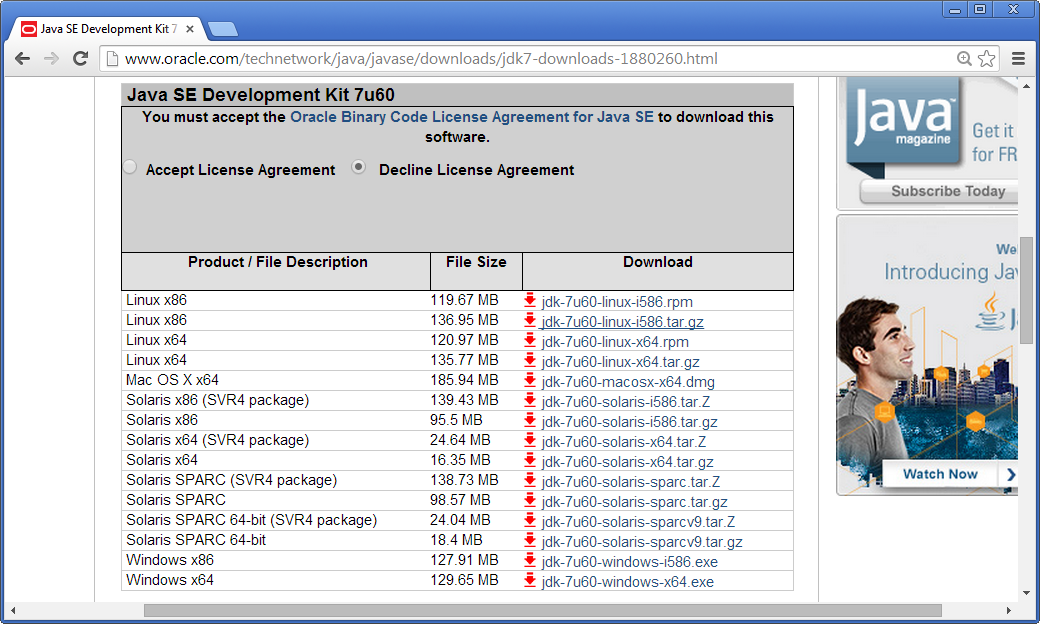
\includegraphics[width=15cm]{oracle_jdk_download.png}
\caption{Installer download for Oracle JDK 7. The Windows 64bit installer package is highlighted.}
\figlabel{jdk_download_oracle}
\end{figure}

Once you have successfully downloaded the JDK installer, follow the Windows installation guide\footnote{
Install the JDK on Windows: \url{http://docs.oracle.com/javase/7/docs/webnotes/install/windows/jdk-installation-windows.html\#Run}}.
To verify the installation you might want to go through this Java ''Hello World!'' 
tutorial\footnote{Windows Java ''Hello World!'': \url{http://docs.oracle.com/javase/tutorial/getStarted/cupojava/win32.html}}.

Installation instructions for Linux\footnote{
Install the JDK on Linux: \url{http://docs.oracle.com/javase/7/docs/webnotes/install/linux/linux-jdk.html}
}
and Mac\footnote{
Install the JDK on Mac: \url{http://docs.oracle.com/javase/7/docs/webnotes/install/mac/mac-jdk.html}.
}
are also available from Oracle.

% --------------------------------------------------------------------------- %
\section{Download and Install Scout}
\seclabel{download_install}

\input{modules/DownloadAndInstallScout}

If you have only installed a single JDK you will not need to change the default \texttt{eclipse.ini} file of your Eclipse installation.
In case you have installed multiple JDKs coming with their individual Java Runtime Environments (JREs), you might want to explicitly specifiy which JRE to use.
Open the file \texttt{eclipse.ini} in a editor of your choice and insert the following two lines at the top of the file:

\begin{lstlisting}[
  language=ini
]
-vm
C:\java\jre7\bin\javaw.exe
\end{lstlisting}

where the second line specifies the exact path to the JRE to be used to start your Eclipse Scout installation.

If you have explicitly specified the JRE to be used you verify this in the running Eclipse installation.
Fist, select the \menu{Help|About Eclipse} to open the about dialog.
Then, click on the \button{Installation Details} and switch to the \tab{Configuration}.
In the long list of system properties you will find lines similar to the ones shown below.

\begin{lstlisting}[
  language=ini
]
*** Date: Donnerstag, 19. Juni 2014 10:37:17 Normalzeit

*** Platform Details:

*** System properties:
...
-vm
C:\java\jre7\bin\javaw.exe
...
sun.java.command=... vm C:\java\jre7\bin\javaw.exe -vmargs ...
\end{lstlisting}

You have now successfully completed the Eclipse Scout installation on your Windows environment.
With this running Scout installation you may skip the following section on how to add Scout to an existing Eclipse installation.

% --------------------------------------------------------------------------- %
\section{Add Scout to your Eclipse Installation}

This section describes the installation of Scout into an existing Eclipse installation.
As the audience of this section is assumed to be familiar with Eclipse, we do not describe how you got your Eclipse installation in the first place.
For the provided screenshots we start from the popular package \textit{Eclipse IDE for Java EE Developers}.

\begin{figure}
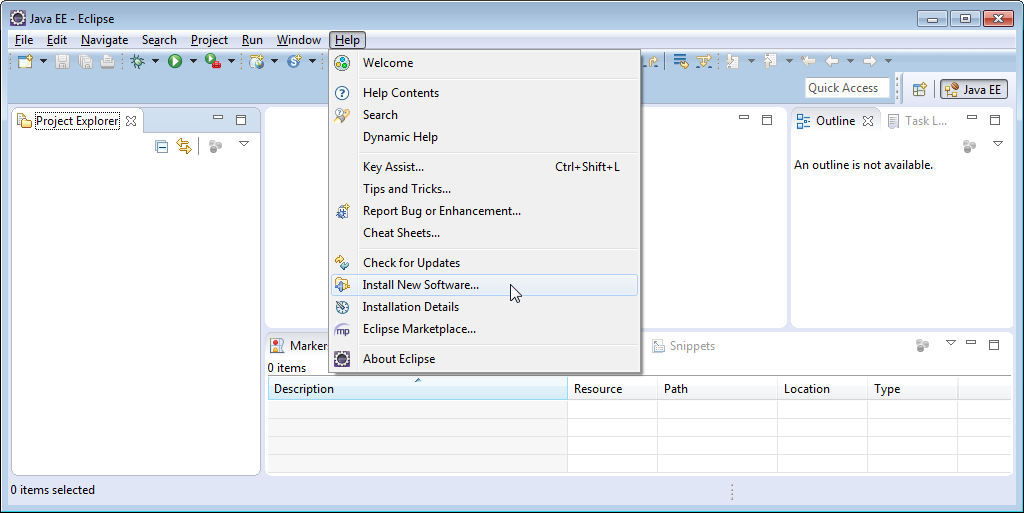
\includegraphics[width=13cm]{eclipse_install_new_software.png}
\caption{Eclipse menu to install additional software}
\figlabel{eclipse_install_new_software}
\end{figure}

To add Scout to your existing Eclipse installation, you need to start Eclipse.
Then select the \menu{Help|Install New Software...} as shown in \figref{eclipse_install_new_software} to open the install dialog.

\begin{figure}
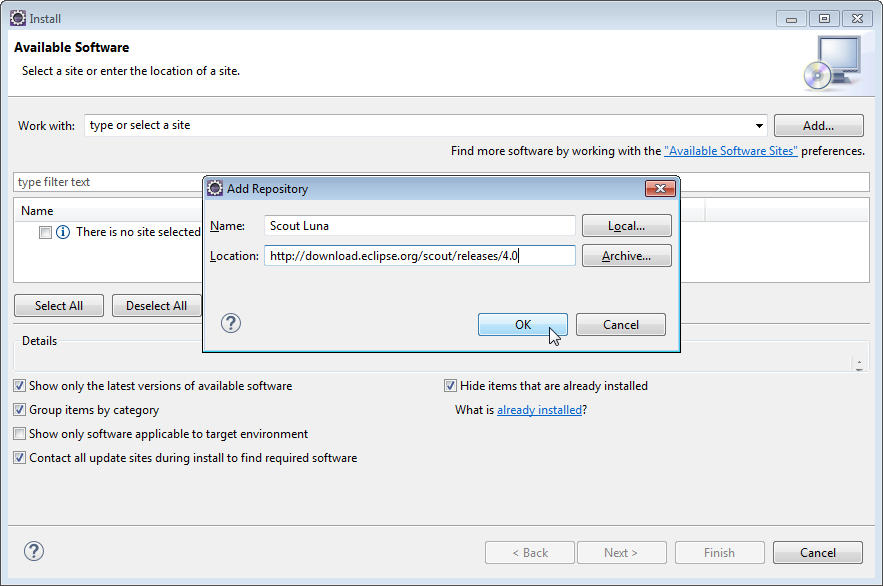
\includegraphics[width=13cm]{eclipse_add_repository.png}
\caption{Add the current Scout repository}
\figlabel{eclipse_add_repository}
\end{figure}

In the install dialog, click on the \button{Add...} to enter the link to the Scout repository.
This opens the popup dialog \textit{Add Repository}
As shown in \figref{eclipse_add_repository}, you may use ''Scout Luna'' for the \field{Name}.
For the \field{Location} enter the Scout release repository as specified below.
\url{http://download.eclipse.org/scout/releases/4.0}.

\begin{figure}
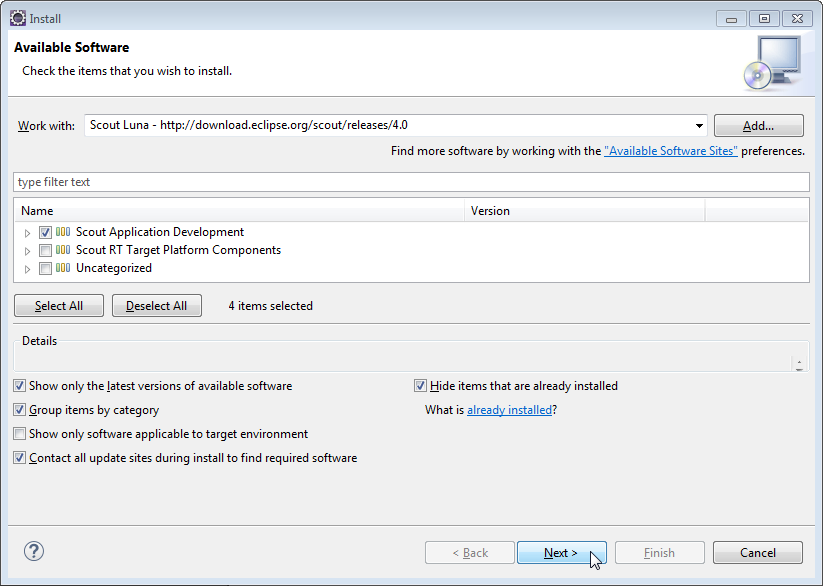
\includegraphics[width=13cm]{eclipse_select_scout_features.png}
\caption{Select the Scout features to add to the Eclipse installation}
\figlabel{eclipse_select_scout_features}
\end{figure}

After the Eclipse IDE has connected to the Scout repository, select the Scout feature \textit{Scout Application Development} as shown in \figref{eclipse_select_scout_features}.
Then, move through the installation with the \button{Next}.
On the last installation step, accept the presented EPL terms by clicking on the appropriate radio button. 
To complete the installation, click the \button{Finish} and accept the request for a restart of Eclipse.
After the restart of the Eclipse IDE, you may add the Scout perspective using the \menu{Window|Open Perspective|Other ...} and selecting the Scout perspective from the presented list. 
Clicking on the Scout perspective button should then result in a state very similar to \figref{scout_perspective}.

% --------------------------------------------------------------------------- %
\section{Verifying the Installation}

After you can start your Eclipse Scout package you need to verify that Scout is working as intended.
The simplest way to verify your Scout installation is to create a ''Hello World'' Scout project and run the corresponding Scout application as described in \charef{helloworld}.

% =========================================================================== %
\chapter{Apache Tomcat Installation}
\applabel{install_tomcat}

Apache Tomcat is an open source web server that is a widely used implementation of the Java Servlet Specification.
Specifically, Tomcat works very well to run the server part of Scout client server applications.
In case you are interested in getting some general context around Tomcat you could start with the Wikipedia article\footnote{
Apache Tomcat Wikipedia: \url{http://en.wikipedia.org/wiki/Apache_Tomcat}.
}.
Then get introduced to its core component ''Tomcat Catalina''\footnote{
Mulesoft's introduction to Tomcat Catalina: \url{http://www.mulesoft.com/tomcat-catalina}.
}
before you switch to the official Tomcat homepage\footnote{
Apache Tomcat Homepage: \url{http://tomcat.apache.org/}
}.

This section is not really a step by step download and installation guide. 
Rather, it points you to the proper places for downloading and installing Tomcat.
We recommend to work with Tomcat version 7.0.
Start your download from the official download site\footnote{
Tomcat 7 Downloads: \url{http://tomcat.apache.org/download-70.cgi}
}.

\begin{figure}
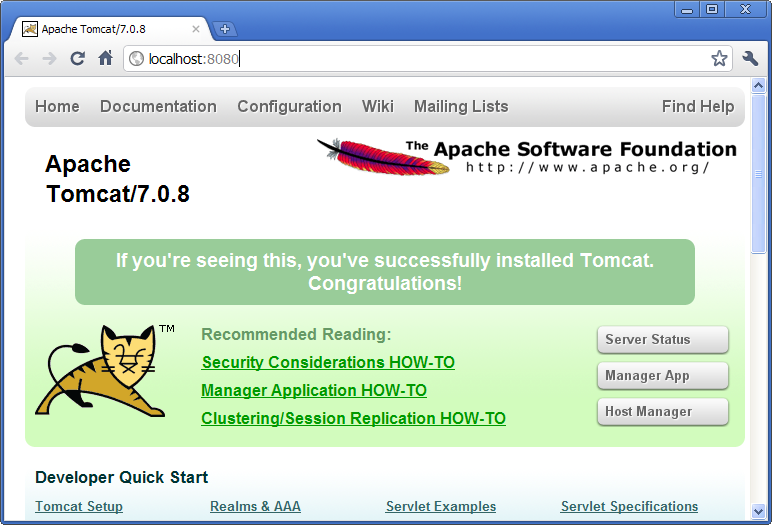
\includegraphics[width=14cm]{tomcat_install.png}
\caption{A successful Tomcat 7 installation.}
\figlabel{tomcat_install}
\end{figure}

Once you have downloaded and installed Tomcat 7 (see the sections below for plattform specific guidelines) you can start the corresponding service or deamon.
To verify that Tomcat is actually running open a web browser of your choice and type \url{http://localhost:8080} into the address bar.
You should then see a confirmation of the successful installation according to \figref{tomcat_install}.

% ........................................................................... %
\section{Platform Specific Instructions}

According to the Tomcat setup installation for Windows\footnote{
Tomcat Windows setup: \url{http://tomcat.apache.org/tomcat-7.0-doc/setup.html\#Windows}
}
download the package ''32-bit/64-bit Windows Service Installer'' from the \href{http://tomcat.apache.org/download-70.cgi}{Tomcat 7 download site}.
Then, start the installer and accept the proposed default settings.

For installing Tomcat on OS X systems download the ''tar.gz'' package from the \href{http://tomcat.apache.org/download-70.cgi}{Tomcat 7 download site}.
Then, follow the installation guide\footnote{
Installing Tomcat on OS X: \url{http://wolfpaulus.com/journal/mac/tomcat7}
} provided by Wolf Paulus.

For Linux systems download the ''tar.gz'' package from the \href{http://tomcat.apache.org/download-70.cgi}{Tomcat 7 download site}.
Then, follow the description of the Unix setup\footnote{
Tomcat Linux setup: \url{http://tomcat.apache.org/tomcat-7.0-doc/setup.html\#Unix_daemon}
}
to run Tomcat as a deamon.
If you use Ubuntu, you may want to follow the tutorial\footnote{
Apache Tomcat Tutorial: \url{http://www.vogella.com/articles/ApacheTomcat/article.html}
} 
for downloading and installing Tomcat provided by Lars Vogel.


% ........................................................................... %
\section{Directories and Files}
\applabel{tomcat_dirs_and_files}

Tomcat's installation directory follows the same organisation on all platforms.
Here, we will only introduce the most important aspects of the Tomcat installation for the purpose of this book.

\begin{figure}
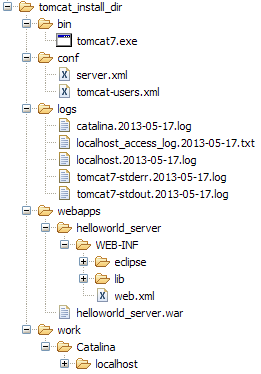
\includegraphics[width=6cm]{tomcat_install_dir.png}
\caption{The organisation of a Tomcat installation including specific files of interest.
As an example, the ''Hello World'' server application is contained in subdirectory \texttt{webapps}.
}
\figlabel{tomcat_install_dir}
\end{figure}

Note that some folders and many files of a Tomcat installation are not represented in \figref{tomcat_install_dir}.
We just want to provide a basic understanding of the most important parts to operate the web server in the context of this book.
In the \filename{bin} folder, the executable programs are contained, including scripts to start and stop the Tomcat instance.

The \filename{conf} folder contains a set of XML and property configuration file.
The file \filename{server.xml} represents Tomcat's main configuration file.
It is used to configure general web server aspects such as the port number of its connectors for the client server communication.
For the default setup, port number 8080 is used for the communication between clients applications and the web server.
The file \filename{tomcat-users.xml} contains a database of users, passwords and associated roles.

Folder \filename{logs} contains various logfiles of Tomcat itself as well as host and web application log files.
XXX need to provide more on what is where (especially application logs and exact setup to generate log entries from scout apps).

The folder needed for deploying web applications into a Tomcat instance is called \filename{webapps}.
It can be used as the target for copying WAR files into the web server.
The installation of the WAR file then extracts its content into the corresponding directory structure as shown in \figref{tomcat_install_dir} in the case of the file \filename{helloworld_server.war}.

Finally, folder \filename{work} contains Tomcat's runtime ''cache'' for the deployed web applications.
It is organized according to the hierarchy of the engine (Catalina), the host (localhost), and the web application (\filename{helloworld_server}).

% ........................................................................... %
\section{The Tomcat Manager Application}
\applabel{tomcat_manager_app}

Tomcat comes with the pre installed ''Manager App''.
This application is useful to manage web applications and perform tasks such as deploying a web application from a WAR file, or starting and stopping installed web applications.
A comprehensive documentation for the ''Manager App'' can be found under the Tomcat homepage\footnote{
The Tomcat Manager Application: \url{http://tomcat.apache.org/tomcat-7.0-doc/manager-howto.html}.
}.
Here we only show how to start this application from the hompage of a running Tomcat installation.

To access this application you can switch to the ''Manager App'' with a click on the corresponding button on the right hand side.
The button can be found on the right hand side of \figref{tomcat_install}.
Before you are allowed to start this application, you need to provide username and password credentials of a user associated with Tomcats's \java{manager-gui} role.

\begin{lstlisting}[
  language=xml,
  float,
  label=\lstlabel{tomcat.users},
  caption=Example content for a \texttt{tomcat-users.xml} file]
  <tomcat-users>
    <!--
    NOTE: By default, no user is included in the "manager-gui" role required
    to operate the "/manager/html" web application. If you wish to use it
    you must define such a user - the username and password are arbitrary.
    -->
	<user name="admin" password="s3cret" roles="manager-gui"/>
  </tomcat-users>	
\end{lstlisting}

To get at user names and passwords you can open file \filename{tomcat-users.xml} located in Tomcat's \filename{conf} directory.
In this file the active users with their passwords and associated roles are stored.
See \lstref{tomcat.users} for an example.
From the content of this file, we see that user \java{admin} has password \java{s3cret} and also posesses the necessary role \java{manager-gui} to access the ''Manager App''.
If file \filename{tomcat-users.xml} does not contain any user with this role, you can simply add new user with this role to the existing users.
Alternatively, you also can add the necessary role to an existing user.
Just append a comma to the existing right(s) followed by the string \java{manager-gui}.
Note that you will need to restart your Tomcat application after adapting the content of file \filename{tomcat-users.xml}.

With working credentials you can now start the ''Manager App'' as described the ''Hello World'' tutorial in \secref{helloworld_deploy}.

% --------------------------------------------------------------------------- %

\ifx\wholebook\relax\else
   \input{../bibliography}
   \end{document}
\fi

% =========================================================================== %
